% Smooth map of manifolds
% Author: Andrew Stacey
% Source: http://www.math.ntnu.no/~stacey/Seminars/ottawa.html
\documentclass{article}
\thispagestyle{empty}
%\def\pgfsysdriver{pgfsys-tex4ht.def}
\usepackage{tikz}
\begin{document}
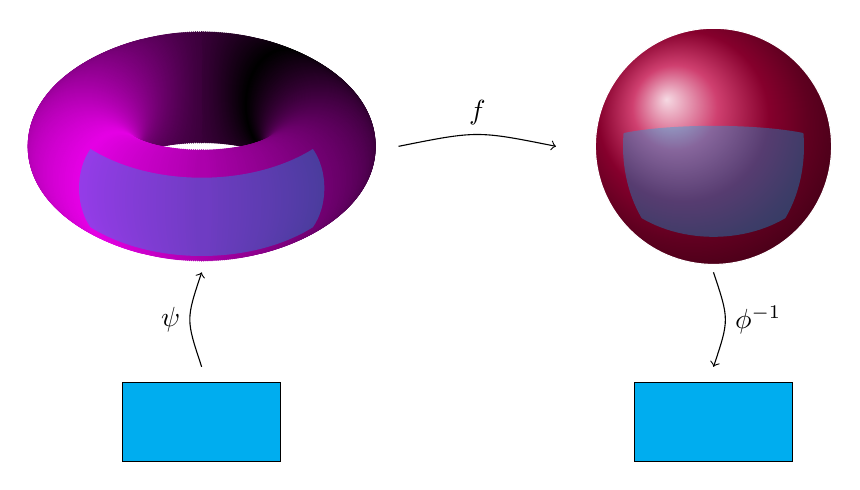
\begin{tikzpicture}
% \x runs over the angles at which to draw the circles defining the
% torus
\foreach \x in {90,89,...,-90} { % change 89 to 80 or 45 for speed
% \elrad is the x-radius of the ellipse (technically, a circle seen
% from side on at angle \x).  The 'max' is because at small angles
% then the real ellipse is too thin and the torus doesn't ``fill
% out'' nicely.
\pgfmathsetmacro\elrad{20*max(cos(\x),.1)}
% We draw the torus from the back to the front to get the right
% layering effect.  To tint it, we define colours according to the
% angle, but need different colours for the left and right pieces.
% It'd be nice if the xcolor colour specification could take something
% computed by pdfmath, such as {red!\tint} but it doesn't appear to
% work, so we define the colours explicitly.
\pgfmathsetmacro\ltint{.9*abs(\x-45)/180}
\pgfmathsetmacro\rtint{.9*(1-abs(\x+45)/180)}
\definecolor{currentcolor}{rgb}{\ltint, 0, \ltint}
% This draws the right-hand circle.
\draw[color=currentcolor,fill=currentcolor] (xyz polar cs:angle=\x,y radius=.75,x radius=1.5) ellipse (\elrad pt and 20pt);
% This sets the colour correctly for the left-hand circle ...
\definecolor{currentcolor}{rgb}{\rtint, 0, \rtint}
% ... and draws it
\draw[color=currentcolor,fill=currentcolor] (xyz polar cs:angle=180-\x,radius=.75,x radius=1.5) ellipse (\elrad pt and 20pt);
% End of foreach statement
}
% Spheres are *much* easier!
\shadedraw[shading=ball,ball color=purple, white] (6.5,0) circle (1.5);
% As are the subsets of Euclidean space
\draw[fill=cyan] (-1,-4) rectangle (1,-3);
\draw[fill=cyan] (5.5,-4) rectangle (7.5,-3);
% The next three draw the maps, slightly curved for aesthetics.
\draw[->] (0,-2.8) .. controls (-.2,-2.2) .. (0,-1.6) node[pos=0.5, auto=left] {\(\psi\)};
\draw[->] (6.5,-1.6) .. controls (6.7,-2.2) .. (6.5,-2.8) node[pos=0.5, auto=left] {\(\phi^{-1}\)};
\draw[->] (2.5,0) .. controls (3.5,.2) .. (4.5,0) node[pos=0.5, auto=left] {\(f\)};
% Now we want to draw the codomains of the charts.  Sticking cosines
% and sines directly into the coordinates doesn't seem to work so
% we define macros to hold the sines and cosines of the angles.
% \elrad is the angle on the torus at which to start.
\pgfmathsetmacro\elrad{cos(-135)}
% the circle drawn at the specific angle on the torus looks like an
% ellipse, \xrad and \yrad compute its major and minor semi-axes.
\pgfmathsetmacro\xrad{1.5cm-20pt*\elrad}
\pgfmathsetmacro\yrad{.75cm-20pt*sin(-135)}
% This draws the codomain of the chart on the torus.
\path[fill=cyan, fill opacity=.35] (xyz polar cs:angle=-135,radius=.75,x radius=1.5) ++(20pt*\elrad,0) arc (0:45:20*\elrad pt and 20pt) arc (-135:-45:\xrad pt and \yrad pt) arc (45:-45:-20*\elrad pt and 20pt) arc (-45:-135:\xrad pt and \yrad pt) arc (-45:0:20*\elrad pt and 20pt);
% Now we do the same for the sphere.
% We do this by drawing some great circles (aka ellipses) on the
% sphere and then ``clipping'' an overlaid (and slightly trans:parent)
% sphere by those great circles.  Each great circle actually specifies
% one side of the ``clip'' so to make sure that the clip is big enough
% the arcs are completed by big rectangles (otherwise the clipping
% would join the end points directly).
\pgfmathsetmacro\tell{-sin(10)}
\pgfmathsetmacro\bell{sin(50)}
\pgfmathsetmacro\rell{1.5 * sin(50)}
\begin{scope}
\clip (6.5,0) +(-1.5,0) arc (-180:0:1.5 and 1.5*\tell) -- ++(0,-1.5) -- ++(-3,0) -- ++(0,1.5);
\clip (6.5,0) +(-1.5,0) arc (-180:0:1.5 and 1.5*\bell) -- ++(0,1.5) -- ++(-3,0) -- ++(0,-1.5);
\clip (6.5,0) +(0,1.5)  arc (90:-90:\rell cm and 1.5 cm) -- ++(-1.5,0) -- ++(0,3) -- ++(1.5,0);
\clip (6.5,0) +(0,1.5)  arc (90:-90:-\rell cm and 1.5 cm) -- ++(1.5,0) -- ++(0,3) -- ++(-1.5,0);
\fill[cyan, fill opacity=0.35] (6.5,0) circle (1.5);
\end{scope}
\end{tikzpicture}
\end{document}
